\documentclass{article}
\usepackage[utf8]{inputenc}
\usepackage[russian]{babel}
\usepackage{graphics}
\usepackage{amsfonts}
\usepackage{amssymb}

\ifx\pdfoutput\undefined
\usepackage{graphicx}
\else
\usepackage[pdftex]{graphicx}
\fi

\hoffset -2.0cm	
\voffset -3.0cm
\textheight 23.5cm 
\textwidth 17.0cm

\title{\bf Лемма о ребрах связующего графа Делоне}
\author{Амосов Федор}

\begin{document}
	\maketitle

    \paragraph{Лемма\\}
        \begin{itemize}
            \item Пусть дан набор $d$--мерных точек $P$, в котором любые $d + 2$ точки не лежат на одной $d$--мерной сфере, и дана точка $q$ вне $Conv P$.
            \item Пусть $D_P$ --- симплексикацию Делоне набора точек $P$. Пусть $D$ --- симплексикация Делоне всех точек ($P \cup \{q\}$).
            \item Назовем симплекс из $D_P$ {\it плохим}, если его описанный шар содержит внутри точку $q$. Назовем {\it связующей} симплексикацию Делоне $D'$, построенную на граничных точках $Conv P$, на вершинах плохих симплексов и на точке $q$. 
            \item Утверждение: множество ребер симплексикации $D$ без ребер $D_P$ совпадает с множеством ребер $D'$, инцендентных вершине $q$.
        \end{itemize}
        
        \begin{center}
	        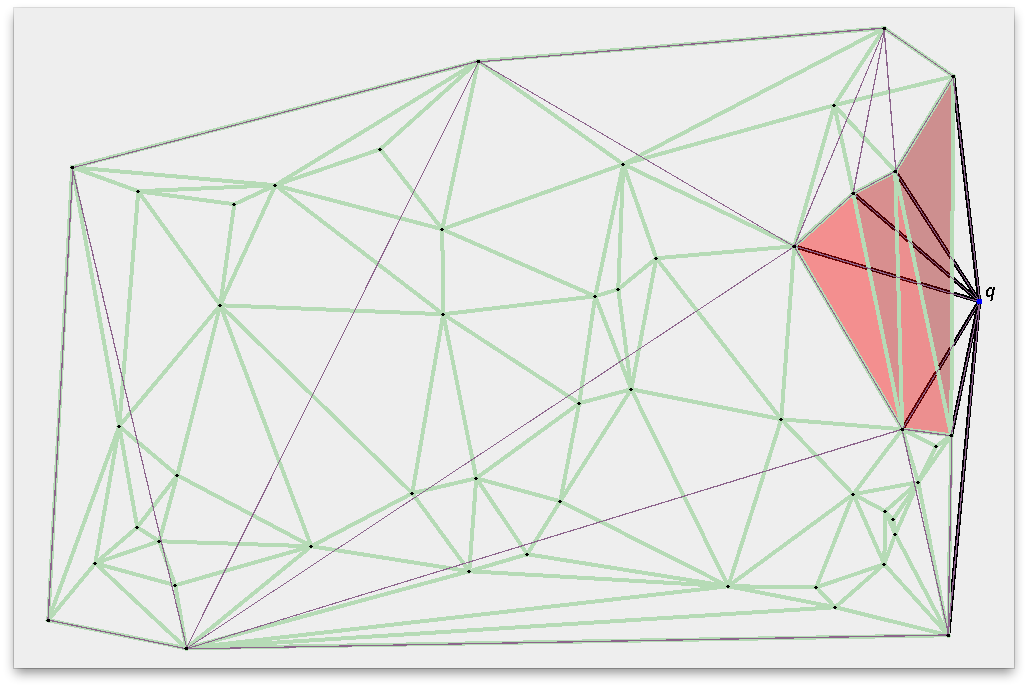
\includegraphics[scale = 0.45]{1.png}
	    \end{center}
        
    \paragraph{Доказательство\\}
        Этот раздел еще не создан.
        %Обозначим множество ребер графа $D$ без ребер графа $D_P$ за $A$, а множество ребер связующего графа $D'$, инцендентных вершине $q$ за $B$.
        
        %Докажем, что $A \subset B$.        
        
        
\end{document}
